\mode*

\section{What's the problem?}

\begin{frame}
  \centering
  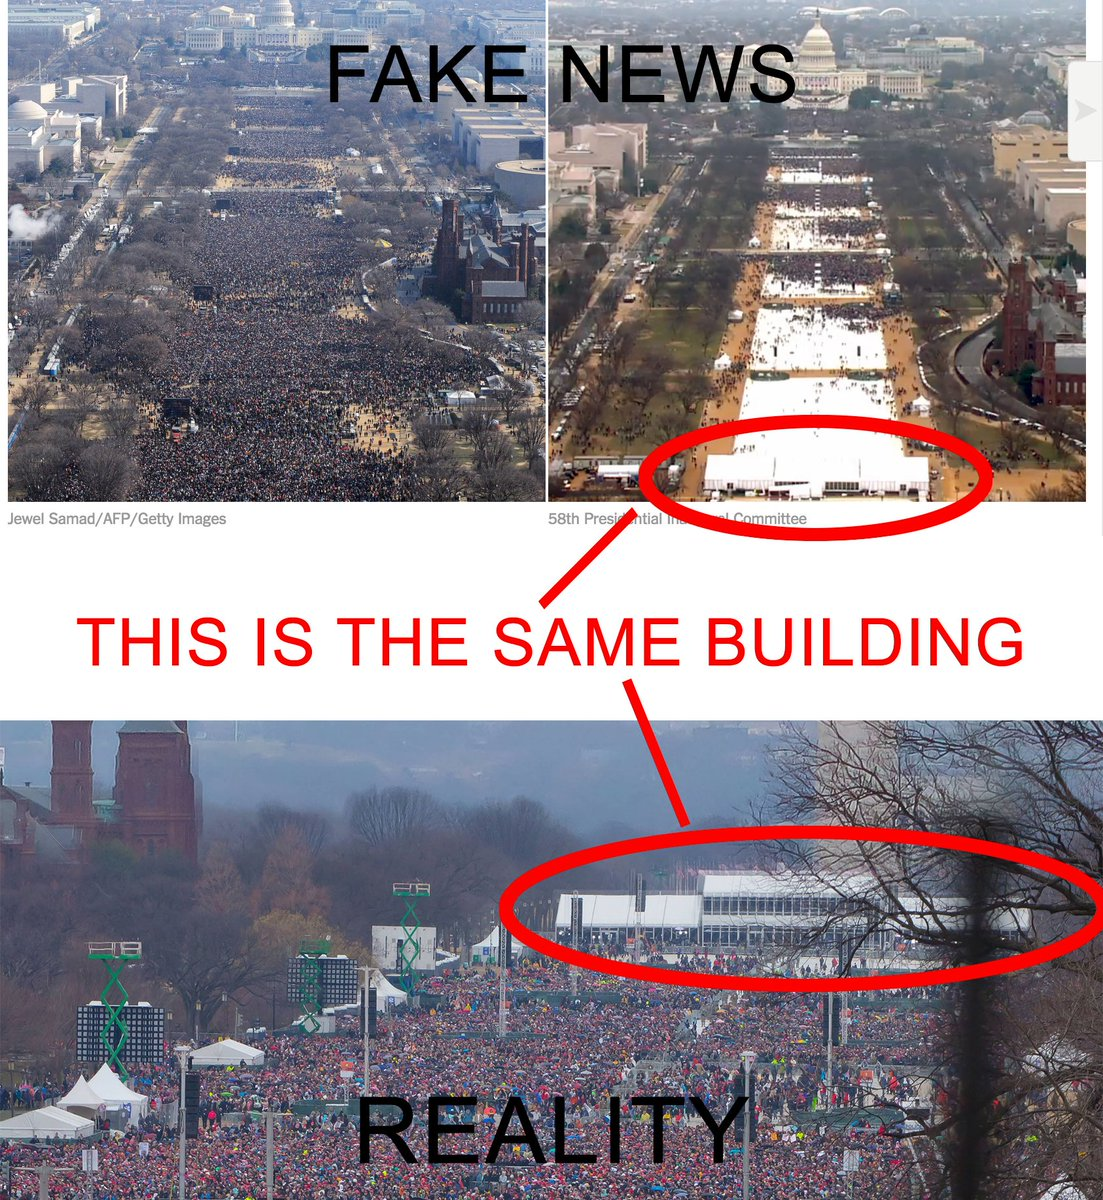
\includegraphics[height=\textheight]{trump.jpg}
\end{frame}


\section[Participating]{Participating in a protest}

\subsection{Joining a protest}

\begin{frame}
  \centering
  \includegraphics[height=0.5\textheight]{ProtestVerif-join.png}
\end{frame}

\subsection{During in a protest}

\begin{frame}
  \centering
  \includegraphics[height=0.5\textheight]{ProtestVerif-participating.png}
\end{frame}

\begin{frame}
  \centering
  \includegraphics{proofshare.tikz}
\end{frame}

\subsection{After the protest}

\begin{frame}
  \centering
  \includegraphics[height=0.5\textheight]{ProtestVerif-endprotest.png}
\end{frame}


\section[Verifying]{Verifying a protest}

\begin{frame}
  \centering
  \includegraphics[height=0.5\textheight]{ProtestVerif-verifying.png}
\end{frame}

\subsection{Verifying proof shares}

\begin{frame}
  \begin{columns}
    \begin{column}{0.6\linewidth}
      \tiny
      \includegraphics[width=\linewidth]{proofshare.tikz}
    \end{column}

    \begin{column}{0.5\linewidth}
      \begin{itemize}
        \item Check that \(cid\) is what you're interested in.
        \item Verify the \ac{NIZK} proofs.
        \item Each \(PRF\) is computed correctly.
        \item The owner knows a signature on the key used.
      \end{itemize}
    \end{column}
  \end{columns}
\end{frame}

\subsection{Counting proofs}

\begin{frame}
  \begin{example}[No trusted witnesses]
    \begin{itemize}
      \item Each \(pid\) with more than \(t\) valid proof shares is counted.
      \item \(t\) is a threshold set to be higher than expected size of collusion 
        clusters.
    \end{itemize}
  \end{example}

  \begin{example}[Trusted witnesses]
    \begin{itemize}
      \item Alternatively, each \(\pid\) with a proof share issued by a trusted 
        witness is counted.
    \end{itemize}
  \end{example}
\end{frame}

\begin{frame}
  \centering
  \includegraphics[height=0.5\textheight]{ProtestVerif-verified.png}
  \includegraphics[height=0.5\textheight]{ProtestVerif-UN.png}
\end{frame}


\begin{figure}
  \centering
  %\footnotesize
  \begin{minipage}{\linewidth}
    \begin{align*}
      O\to \text{all}\colon & \text{manifesto} \\
      P\colon & t_s\gets \TSget \\
        & \cid\gets \Hash[\text{manifesto}], \\
        & \pid\gets \ACprf[_{\sk_P}][\cid] \\
      W\colon & t_s'\gets \TSget
      \\[-1em]
      \noalign{\hfill Join}
      \midrule
      \noalign{\hfill Participation}
      \\[-3em]
      P\to W\colon & \pid \\
      P\leftrightarrow W\colon &
        \PPK\mleft\{ (\sk_P) : \mright. \\
        & \qquad \pid = \ACprf[_{\sk_P}][\cid], \\
        & \qquad \mleft. \sigma_P' = \ACblind[\ACsign[_{\ssk}][\sk_P]] \mright\} 
        \\
      W\colon & \wid\gets \ACprf[_{\sk_W}][\pid] \\
      W\to P\colon & (\wid, t_s', l)
      \\[-1em]
      \noalign{\hfill Participation}
      \midrule
      \noalign{\hfill Submission}
      \\[-2em]
      P\colon & t_e\gets \TSstamp[\Hash[\pid, \wid, t_s, t_s', l]] \\
      W\colon & t_e'\gets \TSstamp[\Hash[\pid, \wid, t_s, t_s', l]] \\
      W\to S\colon & (\pid, \wid, t_s, t_s', t_e, l, \pi_{\wid}),\quad 
      \text{where} \\
        & \pi_{\wid} = \SPK\mleft\{ (\sk_W) : \mright. \\
        & \qquad \wid = \ACprf[_{\sk_W}][\pid], \\
        & \qquad \mleft. \sigma_W' = \ACblind[\ACsign[_{\ssk}][\sk_W]]\mright\} 
        \\
        & \qquad\qquad (\pid, \wid, t_s, t_s', l) \\
      P\to S\colon & (\cid, \pid, \wid, t_s, t_s', t_e, l, \pi_{\pid}),\quad 
      \text{where}\\
        & \pi_{\pid} = \SPK\mleft\{ (\sk_P) : \mright. \\
        & \qquad \pid = \ACprf[_{\sk_P}][\cid], \\
        & \qquad \mleft. \sigma_P' = \ACblind[\ACsign[_{\ssk}][\sk_P]] \mright\} 
        \\
        & \qquad\qquad (\cid, \pid, \wid, t_s, t_s', l)
    \end{align*}
  \end{minipage}
  \caption{%
    An overview of the Join, Participation and Submission phases of \PRIVO.\@
    The organizer \(O\) broadcasts the manifesto.
    The protester \(P\), witness \(W\) and their computations are as in \cref{fig:ProofFig}.
    Finally, both \(P\) and \(W\) submits the proof shares to a permanent storage \(S\).
  }%
  \label{fig:ProtocolOverview}
\end{figure}

\section{Conclusions}

\begin{frame}
  \begin{block}{Contributions}
    \begin{itemize}
      \item Distance-bounding Schnorr protocol
      \item \Ie distance-bounding \acs{ZKP} and anonymous credentials
      \item Solves crowd counting in adversarial setting.
    \end{itemize}
  \end{block}
\end{frame}

\begin{frame}
  \begin{greenblock}{Possibilities}
    \begin{itemize}
      \item We can implement this by extending BankID.
      \item There are blockchains (ledgers) with reasonable transaction 
        throughput, \eg OmniLedger.
    \end{itemize}
  \end{greenblock}

  \begin{alertblock}{Limits}
    \begin{itemize}
      \item Cannot trust results that are pro-government if government issues 
        credentials (Sybil).

      \item Requires a chip in smartphones for distance bounding.
    \end{itemize}
  \end{alertblock}
\end{frame}
